\documentclass{article}

\usepackage{fancyhdr} % Required for custom headers
\usepackage{lastpage} % Required to determine the last page for the footer
\usepackage{extramarks} % Required for headers and footers
\usepackage[usenames,dvipsnames]{color} % Required for custom colors
\usepackage{graphicx} % Required to insert images
\usepackage{listings} % Required for insertion of code
\usepackage{courier} % Required for the courier font
\usepackage{lipsum} % Used for inserting dummy 'Lorem ipsum' text into the template
\usepackage{amsmath}
\usepackage{amssymb}
\usepackage{mathtools, xparse}
\usepackage{booktabs}
\usepackage{bigstrut}
\usepackage{float}
\usepackage{hyperref}
\usepackage{color}
\usepackage{algorithm}
\usepackage{caption}
\usepackage{algpseudocode}
\usepackage{multirow}


\DeclarePairedDelimiter{\norm}{\lVert}{\rVert}
\DeclarePairedDelimiter\abs{\lvert}{\rvert}%

\hypersetup{
    colorlinks   = true,    % Colours links instead of ugly boxes
    urlcolor     = red,    % Colour for external hyperlinks
    linkcolor    = red,    % Colour of internal links
    citecolor    = red      % Colour of citations
}
% Margins
\topmargin=-0.45in
\evensidemargin=0in
\oddsidemargin=0in
\textwidth=6.5in
\textheight=9.0in
\headsep=0.25in

\linespread{1.1} % Line spacing

% Set up the header and footer
\pagestyle{fancy}
\lhead{\hmwkAuthorName} % Top left header
\chead{\hmwkClass\ : \hmwkID} % Top center head
\rhead{\firstxmark} % Top right header
\lfoot{\lastxmark} % Bottom left footer
\cfoot{} % Bottom center footer
\rfoot{Page\ \thepage\ of\ \protect\pageref*{LastPage}} % Bottom right footer
\renewcommand\headrulewidth{0.4pt} % Size of the header rule
\renewcommand\footrulewidth{0.4pt} % Size of the footer rule

\setlength\parindent{0pt} % Removes all indentation from paragraphs

%----------------------------------------------------------------------------------------
%	CODE INCLUSION CONFIGURATION
%----------------------------------------------------------------------------------------

\definecolor{MyDarkGreen}{rgb}{0.0,0.4,0.0} % This is the color used for comments
\lstloadlanguages{Perl} % Load Perl syntax for listings, for a list of other languages supported see: ftp://ftp.tex.ac.uk/tex-archive/macros/latex/contrib/listings/listings.pdf
\lstset{language=Perl, % Use Perl in this example
    frame=single, % Single frame around code
    basicstyle=\small\ttfamily, % Use small true type font
    keywordstyle=[1]\color{Blue}\bf, % Perl functions bold and blue
    keywordstyle=[2]\color{Purple}, % Perl function arguments purple
    keywordstyle=[3]\color{Blue}\underbar, % Custom functions underlined and blue
    identifierstyle=, % Nothing special about identifiers                                         
    commentstyle=\usefont{T1}{pcr}{m}{sl}\color{MyDarkGreen}\small, % Comments small dark green courier font
    stringstyle=\color{Purple}, % Strings are purple
    showstringspaces=false, % Don't put marks in string spaces
    tabsize=5, % 5 spaces per tab
    %
    % Put standard Perl functions not included in the default language here
    morekeywords={rand},
    %
    % Put Perl function parameters here
    morekeywords=[2]{on, off, interp},
    %
    % Put user defined functions here
    morekeywords=[3]{test},
    %
    morecomment=[l][\color{Blue}]{...}, % Line continuation (...) like blue comment
    numbers=left, % Line numbers on left
    firstnumber=1, % Line numbers start with line 1
    numberstyle=\tiny\color{Blue}, % Line numbers are blue and small
    stepnumber=5 % Line numbers go in steps of 5
}

% Creates a new command to include a perl script, the first parameter is the filename of the script (without .pl), the second parameter is the caption
\newcommand{\perlscript}[2]{
    \begin{itemize}
        \item[]\lstinputlisting[caption=#2,label=#1]{#1.py}
    \end{itemize}
}
\newcommand{\cppscript}[1]{
    \begin{itemize}
        \item[]\lstinputlisting[]{#1}
    \end{itemize}
}

%----------------------------------------------------------------------------------------
%	DOCUMENT STRUCTURE COMMANDS
%	Skip this unless you know what you're doing
%----------------------------------------------------------------------------------------

% Header and footer for when a page split occurs within a problem environment
\newcommand{\enterProblemHeader}[1]{
    \nobreak\extramarks{#1}{#1 continued on next page\ldots}\nobreak
    \nobreak\extramarks{#1 (continued)}{#1 continued on next page\ldots}\nobreak
}

% Header and footer for when a page split occurs between problem environments
\newcommand{\exitProblemHeader}[1]{
    \nobreak\extramarks{#1 (continued)}{#1 continued on next page\ldots}\nobreak
    \nobreak\extramarks{#1}{}\nobreak
}

%\setcounter{secnumdepth}{0} % Removes default section numbers
\newcounter{homeworkProblemCounter} % Creates a counter to keep track of the number of problems

\newcommand{\homeworkProblemName}{}
\newenvironment{homeworkProblem}[1][Problem \arabic{homeworkProblemCounter}]{ % Makes a new environment called homeworkProblem which takes 1 argument (custom name) but the default is "Problem #"
    \stepcounter{homeworkProblemCounter} % Increase counter for number of problems
    \renewcommand{\homeworkProblemName}{#1} % Assign \homeworkProblemName the name of the problem
    \section{\homeworkProblemName} % Make a section in the document with the custom problem count
    \enterProblemHeader{\homeworkProblemName} % Header and footer within the environment
    }{
    \exitProblemHeader{\homeworkProblemName} % Header and footer after the environment
}

\newcommand{\problemAnswer}[1]{ % Defines the problem answer command with the content as the only argument
\noindent\framebox[\columnwidth][c]{\begin{minipage}{0.98\columnwidth}#1\end{minipage}} % Makes the box around the problem answer and puts the content inside
}

\newcommand{\homeworkSectionName}{}
\newenvironment{homeworkSection}[1]{ % New environment for sections within homework problems, takes 1 argument - the name of the section
    \renewcommand{\homeworkSectionName}{#1} % Assign \homeworkSectionName to the name of the section from the environment argument
    \subsection{\homeworkSectionName} % Make a subsection with the custom name of the subsection
    \enterProblemHeader{\homeworkProblemName\ [\homeworkSectionName]} % Header and footer within the environment
    }{
    \enterProblemHeader{\homeworkProblemName} % Header and footer after the environment
}

%----------------------------------------------------------------------------------------
%	NAME AND CLASS SECTION
%----------------------------------------------------------------------------------------

\newcommand{\hmwkID}{homework 07} % Assignment title
\newcommand{\hmwkTitle}{Matrix Eigenvalues}
\newcommand{\hmwkDueDate}{Tuesday,\ April\ 18,\ 2017} % Due date
\newcommand{\hmwkClass}{Numerical Analysis} % Course/class
\newcommand{\hmwkClassTime}{10:30am} % Class/lecture time
\newcommand{\hmwkClassInstructor}{Jones} % Teacher/lecturer
\newcommand{\hmwkAuthorName}{102061149 Fu-En Wang} % Your name

%----------------------------------------------------------------------------------------
%	TITLE PAGE
%----------------------------------------------------------------------------------------

\title{
    \vspace{2in}
    \textmd{\textbf{\hmwkClass}}\\
    \textmd{\textbf{\hmwkID: \hmwkTitle}} \\
    \normalsize\vspace{0.1in}\small{Due\ on\ \hmwkDueDate}\\
    \vspace{3in}
}

\author{\textbf{\hmwkAuthorName}}
\date{} % Insert date here if you want it to appear below your name

%----------------------------------------------------------------------------------------

\begin{document}
\maketitle
\newpage

\section{Introduction}
In previous homework, we had already use power method and inverse power method to find the largest and smallest eigenvalue.
However, both of them cannot be used to find all the eigenvalue of a matrix $A$; therefore, it this project, we will use
\textbf{QR Method} to find all the eigenvalues.

\subsection{API}
In \textbf{MAT.h} and \textbf{MAT.cpp}, I implement the following functions:
\begin{enumerate}
    \item \textbf{void QRFact(const MAT \&A, MAT \&Q, MAT \&R);}
    \item \textbf{int EVqr(MAT \&A, double tol, int maxiter);}
    \item \textbf{int EVqrShifted(MAT \&A, double mu, double tol, int maxiter);}
\end{enumerate}
\textbf{QRFact} will apply \textbf{QR Decomposition} to A and store them into Q and R. \textbf{EVqr} and \textbf{EVqrShifted}
is the implementation of \textbf{QR Iteration} and \textbf{Shifted QR Iteration}. In this assignment, \textbf{tol} should be set to
$10^{-9}$ and \textbf{mu} should be 0.5. We have to find the three largest and the three smallest eigenvalues of 
\textbf{m3.dat}, \textbf{m4.dat}, \textbf{m5.dat}, \textbf{m6.dat}, \textbf{m7.dat}, \textbf{m8.dat}.

\subsection{Error Calculation}
According to \textbf{Gram-Schmidt Process}, we should get a final matrix with 0 in the non-diagonal from \textbf{QR Iteration}.
Therefore, it makes sense that we can check whether all non-diagonal elements are zero or not. However, for saving execution
time, we simply this checking to the following fomula:
$$
    error = \max_{2 \leq i \leq n}{\abs{a_{i,i-1}}}
$$
For each iteration, we only check the one-line elements below diagonal, which will be faster a lot than checking all
non-diagonal elements.

\section{Implementation}
\begin{algorithm}[H]
    \caption{\textbf{QR Decomposition}}
    \begin{algorithmic}
        \State $A = \{a_1, a_2, ..., a_n\}, a_i$ is column vector,
        \State $r_{11} = \sqrt{(a_1)^Ta_1}$
        \State $q_1 = \frac{a_1}{r_{11}}$
        \For{each j $\in$ \{2, ..., n\}}
            \State $q_j = a_j$
            \For{each i $\in$ \{1, ..., j-1\}}
                \State $r_{ij} = (q_i)^Tq_j$
                \State $q_j -= r_{ij}q_i$
            \EndFor
            \State $r_{jj} = \sqrt{(q_j)^Tq_j}$
            \State $q_j = \sqrt{sum((q_j)^2)}$
        \EndFor
    \end{algorithmic}
\end{algorithm}
\begin{algorithm}[H]
    \caption{\textbf{QR Iteration}}
    \begin{algorithmic}
        \State $T^{(0)} = A$
        \For{each k $\in$ \{1, ..., maxIter\}}
            \State $T^k = Q^kR^k$
            \State $T^{k+1} = R^kQ^k$
            \If{error $<$ tol}
                \State break
            \EndIf
        \EndFor
    \end{algorithmic}
\end{algorithm}
\begin{algorithm}[H]
    \caption{\textbf{Shifted QR Iteration}}
    \begin{algorithmic}
        \State $T^{(0)} = A$
        \For{each k $\in$ \{1, ..., maxIter\}}
            \State $T^k - {\mu}I = Q^kR^k$
            \State $T^{k+1} = R^kQ^k + {\mu}I$
            \If{error $<$ tol}
                \State break
            \EndIf
        \EndFor
    \end{algorithmic}
\end{algorithm}
\subsection{Complexity}
\label{sec:complexity}
For \textbf{QR Decomposition}, the double for-loop do $\frac{n(n+1)}{2}$ times of operation, and $(q_i)^Tq_j$ in each
operation make \textbf{QR Decomposition} be a {\boldmath$O(n^3)$} problem. \newline
For each iteration of \textbf{QR Iteration}, there are \textbf{QR Decomposition} and \textbf{mat {\boldmath$\times$} mat}. 
So it is also {\boldmath$O(n^3)$} problem.

\section{Discussion}
In the section, we will discuss the following topics:
\begin{enumerate}
    \item Eigenvalues of m3, ..., m15.dat
    \item Runtime of EVqr
    \item Runtime of EVqrShifted
\end{enumerate}

\subsection{Eigenvalues}
Table \ref{tab:eigen evqr} and \ref{tab:eigen evqrshifted} show eigenvalue calculated by \textbf{EVqr} and \textbf{EVqrShifted}, respectively.
\begin{table}[H]
    \begin{center}
        \begin{tabular}{|c|c|c|c|c|c|c|c|}
            \hline
            EVqr & N & E\_large\_1 & E\_large\_2 & E\_large\_3 & E\_small\_1 & E\_small\_2 & E\_small\_3 \\ \hline
            m3 & 3 & 0.627719 & 2 & 6.372281 & 0.627719 & 2 & 6.372281 \\ \hline
            m4 & 10 & 4.455992 & 20.431729 & 67.840399 & 0.512543 & 0.55164 & 0.629808 \\ \hline
            m5 & 20 & 17.235222 & 81.223819 & 270.495189 & 0.503097 & 0.512479 & 0.528819 \\ \hline
            m6 & 30 & 38.53868 & 182.544889 & 608.253606 & 0.501373 & 0.505511 & 0.512543 \\ \hline
            m7 & 40 & 68.364136 & 324.394506 & 1081.115447 & 0.500772 & 0.503093 & 0.507004 \\ \hline
            m8 & 50 & 106.711318 & 506.772618 & 1689.080688 & 0.500494 & 0.501978 & 0.504468 \\ \hline
        \end{tabular}
    \end{center}
    \caption{Eigenvalue of EVqr}
    \label{tab:eigen evqr}
\end{table}
\begin{table}[H]
    \begin{center}
        \begin{tabular}{|c|c|c|c|c|c|c|c|}
            \hline
            EVqrShifted & N & E\_large\_1 & E\_large\_2 & E\_large\_3 & E\_small\_1 & E\_small\_2 & E\_small\_3 \\ \hline
            m3 & 3 & 0.627719 & 2 & 6.372281 & 0.627719 & 2 & 6.372281 \\ \hline
            m4 & 10 & 4.455992 & 20.431729 & 67.840399 & 0.512543 & 0.55164 & 0.629808 \\ \hline
            m5 & 20 & 17.235222 & 81.223819 & 270.495189 & 0.503097 & 0.512479 & 0.528819 \\ \hline
            m6 & 30 & 38.53868 & 182.544889 & 608.253606 & 0.501373 & 0.505511 & 0.512543 \\ \hline
            m7 & 40 & 68.364136 & 324.394506 & 1081.115447 & 0.500772 & 0.503093 & 0.507004 \\ \hline
            m8 & 50 & 106.711318 & 506.772618 & 1689.080688 & 0.500494 & 0.501978 & 0.504468 \\ \hline
            m9 & 60 & 153.580161 & 729.679212 & 2432.149321 & 0.500343 & 0.501373 & 0.503097 \\ \hline
            m10 & 70 & 208.970642 & 993.114283 & 3310.321344 & 0.500252 & 0.501008 & 0.502273 \\ \hline
            m11 & 80 & 272.882751 & 1297.07783 & 4323.596758 & 0.500193 & 0.500772 & 0.501739 \\ \hline
            m12 & 90 & 345.316483 & 1641.569852 & 5471.97556 & 0.500152 & 0.50061 & 0.501373 \\ \hline
            m13 & 100 & 426.271836 & 2026.590348 & 6755.457752 & 0.500123 & 0.500494 & 0.501112 \\ \hline
            m14 & 120 & 613.747401 & 2918.216761 & 9727.732302 & 0.500086 & 0.500343 & 0.500772 \\ \hline
            m15 & 150 & 958.872886 & 4559.619934 & 15199.419543 & 0.500055 & 0.500219 & 0.500494 \\ \hline
        \end{tabular}
    \end{center}
    \caption{Eigenvalue of EVqrShifted}
    \label{tab:eigen evqrshifted}
\end{table}

\subsection{EVqr}
Table \ref{tab:iter evqr} show the average iteration time(\textbf{iter\_avg}) and iteration number(\textbf{iter\_num})
for m3 ..... m8.dat.
\begin{table}[H]
    \begin{center}
        \begin{tabular}{|c|c|c|c|c|}
            \hline
            EVqr & N & iter\_num & runtime(s) & iter\_avg \\ \hline
            m3 & 3 & 20 & 7.20E-05 & 3.6000E-06 \\ \hline
            m4 & 10 & 249 & 0.005884 & 2.3631E-05 \\ \hline
            m5 & 20 & 909 & 0.110081 & 1.2110E-04 \\ \hline
            m6 & 30 & 1942 & 0.693329 & 3.5702E-04 \\ \hline
            m7 & 40 & 3325 & 2.88519 & 8.6773E-04 \\ \hline
            m8 & 50 & 5041 & 9.79014 & 1.9421E-03 \\ \hline
        \end{tabular}
    \end{center}
    \caption{Itertion number and iter\_avg of EVqr}
    \label{tab:iter evqr}
\end{table}
From Table \ref{tab:iter evqr}, we can plot iter\_avg vs N and iter\_num vs N as shown in Figure \ref{fig:iter avg evqr} and \ref{fig:iter num evqr}.
\begin{figure}[H]
    \centering
    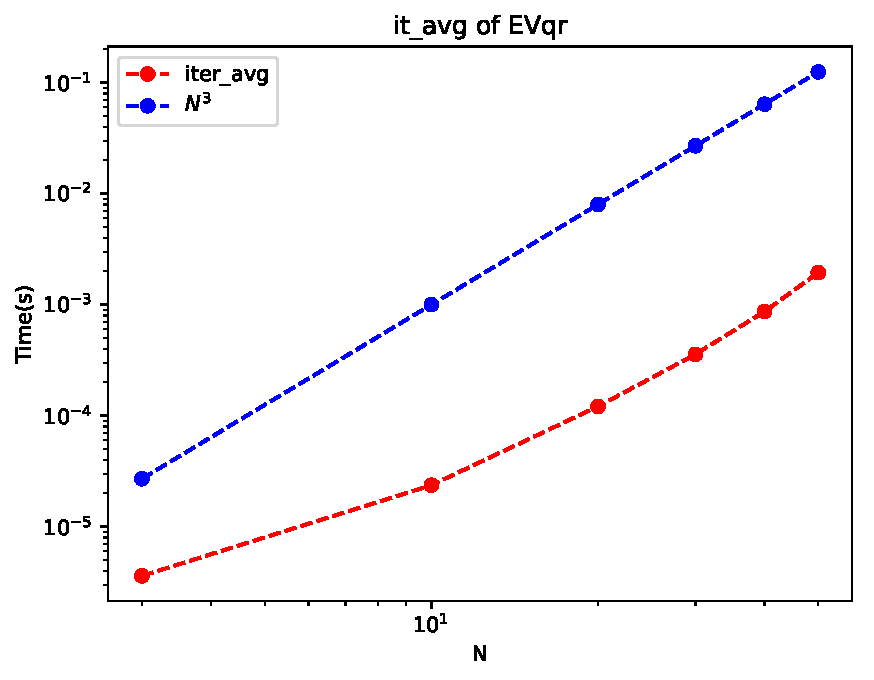
\includegraphics[width=0.6\textwidth]{src/iter_avg_unshifted.pdf}
    \caption{iter\_avg vs N(EVqr)}
    \label{fig:iter avg evqr}
\end{figure}
In Figure \ref{fig:iter avg evqr}, we can find that the slope of iter\_avg is same as $N^3$, which means the complexity of each iteration of
EVqr is {\boldmath$O(n^3)$} and satisfies my analysis in Section \ref{sec:complexity}.
\begin{figure}[H]
    \centering
    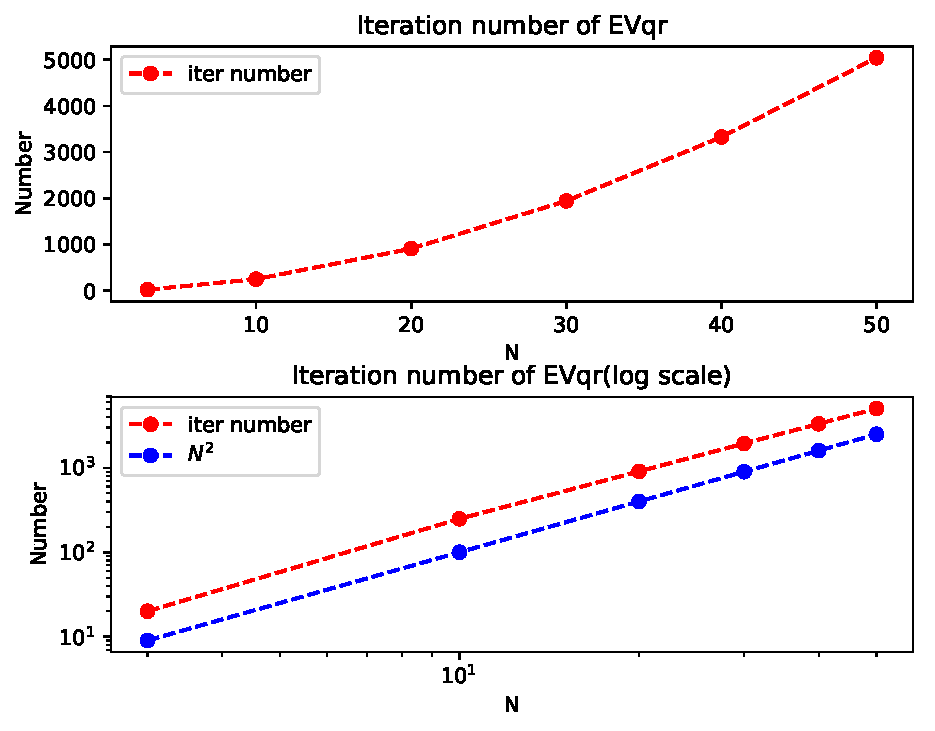
\includegraphics[width=0.7\textwidth]{src/iter_num_unshifted.pdf}
    \caption{iter\_num vs N(EVqr) in normal scale(top) and log scale(bottom)}
    \label{fig:iter num evqr}
\end{figure}


\end{document}













